\documentclass[twoside]{book}

% Packages required by doxygen
\usepackage{calc}
\usepackage{doxygen}
\usepackage{graphicx}
\usepackage[utf8]{inputenc}
\usepackage{makeidx}
\usepackage{multicol}
\usepackage{multirow}
\usepackage{textcomp}
\usepackage[table]{xcolor}

% Font selection
\usepackage[T1]{fontenc}
\usepackage{mathptmx}
\usepackage[scaled=.90]{helvet}
\usepackage{courier}
\usepackage{amssymb}
\usepackage{sectsty}
\renewcommand{\familydefault}{\sfdefault}
\allsectionsfont{%
  \fontseries{bc}\selectfont%
  \color{darkgray}%
}
\renewcommand{\DoxyLabelFont}{%
  \fontseries{bc}\selectfont%
  \color{darkgray}%
}

% Page & text layout
\usepackage{geometry}
\geometry{%
  a4paper,%
  top=2.5cm,%
  bottom=2.5cm,%
  left=2.5cm,%
  right=2.5cm%
}
\tolerance=750
\hfuzz=15pt
\hbadness=750
\setlength{\emergencystretch}{15pt}
\setlength{\parindent}{0cm}
\setlength{\parskip}{0.2cm}
\makeatletter
\renewcommand{\paragraph}{%
  \@startsection{paragraph}{4}{0ex}{-1.0ex}{1.0ex}{%
    \normalfont\normalsize\bfseries\SS@parafont%
  }%
}
\renewcommand{\subparagraph}{%
  \@startsection{subparagraph}{5}{0ex}{-1.0ex}{1.0ex}{%
    \normalfont\normalsize\bfseries\SS@subparafont%
  }%
}
\makeatother

% Headers & footers
\usepackage{fancyhdr}
\pagestyle{fancyplain}
\fancyhead[LE]{\fancyplain{}{\bfseries\thepage}}
\fancyhead[CE]{\fancyplain{}{}}
\fancyhead[RE]{\fancyplain{}{\bfseries\leftmark}}
\fancyhead[LO]{\fancyplain{}{\bfseries\rightmark}}
\fancyhead[CO]{\fancyplain{}{}}
\fancyhead[RO]{\fancyplain{}{\bfseries\thepage}}
\fancyfoot[LE]{\fancyplain{}{}}
\fancyfoot[CE]{\fancyplain{}{}}
\fancyfoot[RE]{\fancyplain{}{\bfseries\scriptsize Generated on Thu May 1 2014 12\-:44\-:50 for Shizuka by Doxygen }}
\fancyfoot[LO]{\fancyplain{}{\bfseries\scriptsize Generated on Thu May 1 2014 12\-:44\-:50 for Shizuka by Doxygen }}
\fancyfoot[CO]{\fancyplain{}{}}
\fancyfoot[RO]{\fancyplain{}{}}
\renewcommand{\footrulewidth}{0.4pt}
\renewcommand{\chaptermark}[1]{%
  \markboth{#1}{}%
}
\renewcommand{\sectionmark}[1]{%
  \markright{\thesection\ #1}%
}

% Indices & bibliography
\usepackage{natbib}
\usepackage[titles]{tocloft}
\setcounter{tocdepth}{3}
\setcounter{secnumdepth}{5}
\makeindex

% Hyperlinks (required, but should be loaded last)
\usepackage{ifpdf}
\ifpdf
  \usepackage[pdftex,pagebackref=true]{hyperref}
\else
  \usepackage[ps2pdf,pagebackref=true]{hyperref}
\fi
\hypersetup{%
  colorlinks=true,%
  linkcolor=blue,%
  citecolor=blue,%
  unicode%
}

% Custom commands
\newcommand{\clearemptydoublepage}{%
  \newpage{\pagestyle{empty}\cleardoublepage}%
}


%===== C O N T E N T S =====

\begin{document}

% Titlepage & ToC
\hypersetup{pageanchor=false}
\pagenumbering{roman}
\begin{titlepage}
\vspace*{7cm}
\begin{center}%
{\Large Shizuka }\\
\vspace*{1cm}
{\large Generated by Doxygen 1.8.5}\\
\vspace*{0.5cm}
{\small Thu May 1 2014 12:44:50}\\
\end{center}
\end{titlepage}
\clearemptydoublepage
\tableofcontents
\clearemptydoublepage
\pagenumbering{arabic}
\hypersetup{pageanchor=true}

%--- Begin generated contents ---
\chapter{Main Page}
\label{index}\hypertarget{index}{}A Client/\-Server application for monitoring a network of computers.

\section*{Features}


\begin{DoxyEnumerate}
\item Remotely monitor networked computer statistics such as C\-P\-U usage, R\-A\-M Usage, network throughput, and uptime.
\item Get Notified by E-\/mail when events are triggered(R\-A\-M/\-C\-P\-U Usage goes over a threshold).
\item Perform a limited set of commands on remote computers from the command page.
\item View on the go with the Mobile App. 
\end{DoxyEnumerate}
\chapter{Namespace Index}
\section{Packages}
Here are the packages with brief descriptions (if available)\-:\begin{DoxyCompactList}
\item\contentsline{section}{\hyperlink{namespaceclient}{client} }{\pageref{namespaceclient}}{}
\item\contentsline{section}{\hyperlink{namespaceclient_1_1_r_a_m_monitor}{client.\-R\-A\-M\-Monitor} }{\pageref{namespaceclient_1_1_r_a_m_monitor}}{}
\item\contentsline{section}{\hyperlink{namespaceclient_1_1_resource_tests}{client.\-Resource\-Tests} }{\pageref{namespaceclient_1_1_resource_tests}}{}
\end{DoxyCompactList}

\chapter{Hierarchical Index}
\section{Class Hierarchy}
This inheritance list is sorted roughly, but not completely, alphabetically\-:\begin{DoxyCompactList}
\item \contentsline{section}{client.\-R\-A\-M\-Monitor.\-R\-A\-M\-Monitor}{\pageref{classclient_1_1_r_a_m_monitor_1_1_r_a_m_monitor}}{}
\item Test\-Case\begin{DoxyCompactList}
\item \contentsline{section}{client.\-Resource\-Tests.\-Test\-Resource\-Monitors}{\pageref{classclient_1_1_resource_tests_1_1_test_resource_monitors}}{}
\end{DoxyCompactList}
\end{DoxyCompactList}

\chapter{Class Index}
\section{Class List}
Here are the classes, structs, unions and interfaces with brief descriptions\-:\begin{DoxyCompactList}
\item\contentsline{section}{\hyperlink{classclient_1_1_r_a_m_monitor_1_1_r_a_m_monitor}{client.\-R\-A\-M\-Monitor.\-R\-A\-M\-Monitor} }{\pageref{classclient_1_1_r_a_m_monitor_1_1_r_a_m_monitor}}{}
\item\contentsline{section}{\hyperlink{classclient_1_1_resource_tests_1_1_test_resource_monitors}{client.\-Resource\-Tests.\-Test\-Resource\-Monitors} }{\pageref{classclient_1_1_resource_tests_1_1_test_resource_monitors}}{}
\end{DoxyCompactList}

\chapter{File Index}
\section{File List}
Here is a list of all files with brief descriptions\-:\begin{DoxyCompactList}
\item\contentsline{section}{C\-:/\-Users/\-Master/\-Documents/\-Git\-Hub/\-Shizuka/src/client/\hyperlink{____init_____8py}{\-\_\-\-\_\-init\-\_\-\-\_\-.\-py} }{\pageref{____init_____8py}}{}
\item\contentsline{section}{C\-:/\-Users/\-Master/\-Documents/\-Git\-Hub/\-Shizuka/src/client/\hyperlink{_r_a_m_monitor_8py}{R\-A\-M\-Monitor.\-py} }{\pageref{_r_a_m_monitor_8py}}{}
\item\contentsline{section}{C\-:/\-Users/\-Master/\-Documents/\-Git\-Hub/\-Shizuka/src/client/\hyperlink{_resource_tests_8py}{Resource\-Tests.\-py} }{\pageref{_resource_tests_8py}}{}
\end{DoxyCompactList}

\chapter{Namespace Documentation}
\hypertarget{namespaceclient}{\section{client Namespace Reference}
\label{namespaceclient}\index{client@{client}}
}
\subsection*{Namespaces}
\begin{DoxyCompactItemize}
\item 
\hyperlink{namespaceclient_1_1_r_a_m_monitor}{R\-A\-M\-Monitor}
\item 
\hyperlink{namespaceclient_1_1_resource_tests}{Resource\-Tests}
\end{DoxyCompactItemize}
\subsection*{Variables}
\begin{DoxyCompactItemize}
\item 
string \hyperlink{namespaceclient_a79ecd5be35a04c57f542965e484a29c0}{\-\_\-\-\_\-author\-\_\-\-\_\-} = 'Master'
\end{DoxyCompactItemize}


\subsection{Variable Documentation}
\hypertarget{namespaceclient_a79ecd5be35a04c57f542965e484a29c0}{\index{client@{client}!\-\_\-\-\_\-author\-\_\-\-\_\-@{\-\_\-\-\_\-author\-\_\-\-\_\-}}
\index{\-\_\-\-\_\-author\-\_\-\-\_\-@{\-\_\-\-\_\-author\-\_\-\-\_\-}!client@{client}}
\subsubsection[{\-\_\-\-\_\-author\-\_\-\-\_\-}]{\setlength{\rightskip}{0pt plus 5cm}string client.\-\_\-\-\_\-author\-\_\-\-\_\- = 'Master'}}\label{namespaceclient_a79ecd5be35a04c57f542965e484a29c0}


Definition at line 1 of file \-\_\-\-\_\-init\-\_\-\-\_\-.\-py.


\hypertarget{namespaceclient_1_1_r_a_m_monitor}{\section{client.\-R\-A\-M\-Monitor Namespace Reference}
\label{namespaceclient_1_1_r_a_m_monitor}\index{client.\-R\-A\-M\-Monitor@{client.\-R\-A\-M\-Monitor}}
}
\subsection*{Classes}
\begin{DoxyCompactItemize}
\item 
class \hyperlink{classclient_1_1_r_a_m_monitor_1_1_r_a_m_monitor}{R\-A\-M\-Monitor}
\end{DoxyCompactItemize}

\hypertarget{namespaceclient_1_1_resource_tests}{\section{client.\-Resource\-Tests Namespace Reference}
\label{namespaceclient_1_1_resource_tests}\index{client.\-Resource\-Tests@{client.\-Resource\-Tests}}
}
\subsection*{Classes}
\begin{DoxyCompactItemize}
\item 
class \hyperlink{classclient_1_1_resource_tests_1_1_test_resource_monitors}{Test\-Resource\-Monitors}
\end{DoxyCompactItemize}
\subsection*{Variables}
\begin{DoxyCompactItemize}
\item 
string \hyperlink{namespaceclient_1_1_resource_tests_a69befa02aa81b89c00cad77ab29d88bb}{\-\_\-\-\_\-author\-\_\-\-\_\-} = 'Tadgh'
\end{DoxyCompactItemize}


\subsection{Variable Documentation}
\hypertarget{namespaceclient_1_1_resource_tests_a69befa02aa81b89c00cad77ab29d88bb}{\index{client\-::\-Resource\-Tests@{client\-::\-Resource\-Tests}!\-\_\-\-\_\-author\-\_\-\-\_\-@{\-\_\-\-\_\-author\-\_\-\-\_\-}}
\index{\-\_\-\-\_\-author\-\_\-\-\_\-@{\-\_\-\-\_\-author\-\_\-\-\_\-}!client::ResourceTests@{client\-::\-Resource\-Tests}}
\subsubsection[{\-\_\-\-\_\-author\-\_\-\-\_\-}]{\setlength{\rightskip}{0pt plus 5cm}string client.\-Resource\-Tests.\-\_\-\-\_\-author\-\_\-\-\_\- = 'Tadgh'}}\label{namespaceclient_1_1_resource_tests_a69befa02aa81b89c00cad77ab29d88bb}


Definition at line 7 of file Resource\-Tests.\-py.


\chapter{Class Documentation}
\hypertarget{classclient_1_1_r_a_m_monitor_1_1_r_a_m_monitor}{\section{client.\-R\-A\-M\-Monitor.\-R\-A\-M\-Monitor Class Reference}
\label{classclient_1_1_r_a_m_monitor_1_1_r_a_m_monitor}\index{client.\-R\-A\-M\-Monitor.\-R\-A\-M\-Monitor@{client.\-R\-A\-M\-Monitor.\-R\-A\-M\-Monitor}}
}
\subsection*{Public Member Functions}
\begin{DoxyCompactItemize}
\item 
def \hyperlink{classclient_1_1_r_a_m_monitor_1_1_r_a_m_monitor_a1029eb60172e2d71eed490f30a68428a}{\-\_\-\-\_\-init\-\_\-\-\_\-}
\item 
def \hyperlink{classclient_1_1_r_a_m_monitor_1_1_r_a_m_monitor_ad225968bc7055e1a98e511d24022551b}{get\-\_\-ram\-\_\-percent}
\end{DoxyCompactItemize}


\subsection{Detailed Description}
\begin{DoxyVerb}This class handles RAM Resource monitoring.
@author Gary Graham
\end{DoxyVerb}
 

Definition at line 4 of file R\-A\-M\-Monitor.\-py.



\subsection{Constructor \& Destructor Documentation}
\hypertarget{classclient_1_1_r_a_m_monitor_1_1_r_a_m_monitor_a1029eb60172e2d71eed490f30a68428a}{\index{client\-::\-R\-A\-M\-Monitor\-::\-R\-A\-M\-Monitor@{client\-::\-R\-A\-M\-Monitor\-::\-R\-A\-M\-Monitor}!\-\_\-\-\_\-init\-\_\-\-\_\-@{\-\_\-\-\_\-init\-\_\-\-\_\-}}
\index{\-\_\-\-\_\-init\-\_\-\-\_\-@{\-\_\-\-\_\-init\-\_\-\-\_\-}!client::RAMMonitor::RAMMonitor@{client\-::\-R\-A\-M\-Monitor\-::\-R\-A\-M\-Monitor}}
\subsubsection[{\-\_\-\-\_\-init\-\_\-\-\_\-}]{\setlength{\rightskip}{0pt plus 5cm}def client.\-R\-A\-M\-Monitor.\-R\-A\-M\-Monitor.\-\_\-\-\_\-init\-\_\-\-\_\- (
\begin{DoxyParamCaption}
\item[{}]{self}
\end{DoxyParamCaption}
)}}\label{classclient_1_1_r_a_m_monitor_1_1_r_a_m_monitor_a1029eb60172e2d71eed490f30a68428a}


Definition at line 11 of file R\-A\-M\-Monitor.\-py.



\subsection{Member Function Documentation}
\hypertarget{classclient_1_1_r_a_m_monitor_1_1_r_a_m_monitor_ad225968bc7055e1a98e511d24022551b}{\index{client\-::\-R\-A\-M\-Monitor\-::\-R\-A\-M\-Monitor@{client\-::\-R\-A\-M\-Monitor\-::\-R\-A\-M\-Monitor}!get\-\_\-ram\-\_\-percent@{get\-\_\-ram\-\_\-percent}}
\index{get\-\_\-ram\-\_\-percent@{get\-\_\-ram\-\_\-percent}!client::RAMMonitor::RAMMonitor@{client\-::\-R\-A\-M\-Monitor\-::\-R\-A\-M\-Monitor}}
\subsubsection[{get\-\_\-ram\-\_\-percent}]{\setlength{\rightskip}{0pt plus 5cm}def client.\-R\-A\-M\-Monitor.\-R\-A\-M\-Monitor.\-get\-\_\-ram\-\_\-percent (
\begin{DoxyParamCaption}
\item[{}]{self}
\end{DoxyParamCaption}
)}}\label{classclient_1_1_r_a_m_monitor_1_1_r_a_m_monitor_ad225968bc7055e1a98e511d24022551b}
\begin{DoxyVerb}This function returns the ram usage as a float from 0.0 to 100.0.
@return float 0.0 <= number <= 100.0
\end{DoxyVerb}
 

Definition at line 15 of file R\-A\-M\-Monitor.\-py.



The documentation for this class was generated from the following file\-:\begin{DoxyCompactItemize}
\item 
C\-:/\-Users/\-Master/\-Documents/\-Git\-Hub/\-Shizuka/src/client/\hyperlink{_r_a_m_monitor_8py}{R\-A\-M\-Monitor.\-py}\end{DoxyCompactItemize}

\hypertarget{classclient_1_1_resource_tests_1_1_test_resource_monitors}{\section{client.\-Resource\-Tests.\-Test\-Resource\-Monitors Class Reference}
\label{classclient_1_1_resource_tests_1_1_test_resource_monitors}\index{client.\-Resource\-Tests.\-Test\-Resource\-Monitors@{client.\-Resource\-Tests.\-Test\-Resource\-Monitors}}
}
Inheritance diagram for client.\-Resource\-Tests.\-Test\-Resource\-Monitors\-:\begin{figure}[H]
\begin{center}
\leavevmode
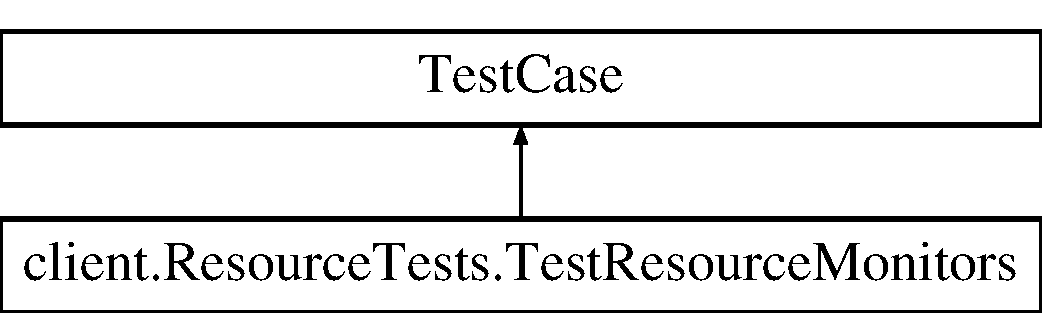
\includegraphics[height=2.000000cm]{classclient_1_1_resource_tests_1_1_test_resource_monitors}
\end{center}
\end{figure}
\subsection*{Public Member Functions}
\begin{DoxyCompactItemize}
\item 
def \hyperlink{classclient_1_1_resource_tests_1_1_test_resource_monitors_ab39ef38db6a8422245ebb58a0aad1db2}{set\-Up}
\item 
def \hyperlink{classclient_1_1_resource_tests_1_1_test_resource_monitors_ab27fab69129411326058cca6a963e5f6}{test\-\_\-ps\-\_\-utils\-\_\-exists}
\item 
def \hyperlink{classclient_1_1_resource_tests_1_1_test_resource_monitors_a31da9c5ac8a67e38738e14dc4a7e4fe5}{test\-\_\-ram\-\_\-reporting}
\end{DoxyCompactItemize}
\subsection*{Public Attributes}
\begin{DoxyCompactItemize}
\item 
\hyperlink{classclient_1_1_resource_tests_1_1_test_resource_monitors_af0a3e8989c7566318eba78dea04849a4}{ram\-\_\-monitor}
\end{DoxyCompactItemize}


\subsection{Detailed Description}


Definition at line 10 of file Resource\-Tests.\-py.



\subsection{Member Function Documentation}
\hypertarget{classclient_1_1_resource_tests_1_1_test_resource_monitors_ab39ef38db6a8422245ebb58a0aad1db2}{\index{client\-::\-Resource\-Tests\-::\-Test\-Resource\-Monitors@{client\-::\-Resource\-Tests\-::\-Test\-Resource\-Monitors}!set\-Up@{set\-Up}}
\index{set\-Up@{set\-Up}!client::ResourceTests::TestResourceMonitors@{client\-::\-Resource\-Tests\-::\-Test\-Resource\-Monitors}}
\subsubsection[{set\-Up}]{\setlength{\rightskip}{0pt plus 5cm}def client.\-Resource\-Tests.\-Test\-Resource\-Monitors.\-set\-Up (
\begin{DoxyParamCaption}
\item[{}]{self}
\end{DoxyParamCaption}
)}}\label{classclient_1_1_resource_tests_1_1_test_resource_monitors_ab39ef38db6a8422245ebb58a0aad1db2}


Definition at line 12 of file Resource\-Tests.\-py.

\hypertarget{classclient_1_1_resource_tests_1_1_test_resource_monitors_ab27fab69129411326058cca6a963e5f6}{\index{client\-::\-Resource\-Tests\-::\-Test\-Resource\-Monitors@{client\-::\-Resource\-Tests\-::\-Test\-Resource\-Monitors}!test\-\_\-ps\-\_\-utils\-\_\-exists@{test\-\_\-ps\-\_\-utils\-\_\-exists}}
\index{test\-\_\-ps\-\_\-utils\-\_\-exists@{test\-\_\-ps\-\_\-utils\-\_\-exists}!client::ResourceTests::TestResourceMonitors@{client\-::\-Resource\-Tests\-::\-Test\-Resource\-Monitors}}
\subsubsection[{test\-\_\-ps\-\_\-utils\-\_\-exists}]{\setlength{\rightskip}{0pt plus 5cm}def client.\-Resource\-Tests.\-Test\-Resource\-Monitors.\-test\-\_\-ps\-\_\-utils\-\_\-exists (
\begin{DoxyParamCaption}
\item[{}]{self}
\end{DoxyParamCaption}
)}}\label{classclient_1_1_resource_tests_1_1_test_resource_monitors_ab27fab69129411326058cca6a963e5f6}


Definition at line 15 of file Resource\-Tests.\-py.

\hypertarget{classclient_1_1_resource_tests_1_1_test_resource_monitors_a31da9c5ac8a67e38738e14dc4a7e4fe5}{\index{client\-::\-Resource\-Tests\-::\-Test\-Resource\-Monitors@{client\-::\-Resource\-Tests\-::\-Test\-Resource\-Monitors}!test\-\_\-ram\-\_\-reporting@{test\-\_\-ram\-\_\-reporting}}
\index{test\-\_\-ram\-\_\-reporting@{test\-\_\-ram\-\_\-reporting}!client::ResourceTests::TestResourceMonitors@{client\-::\-Resource\-Tests\-::\-Test\-Resource\-Monitors}}
\subsubsection[{test\-\_\-ram\-\_\-reporting}]{\setlength{\rightskip}{0pt plus 5cm}def client.\-Resource\-Tests.\-Test\-Resource\-Monitors.\-test\-\_\-ram\-\_\-reporting (
\begin{DoxyParamCaption}
\item[{}]{self}
\end{DoxyParamCaption}
)}}\label{classclient_1_1_resource_tests_1_1_test_resource_monitors_a31da9c5ac8a67e38738e14dc4a7e4fe5}


Definition at line 20 of file Resource\-Tests.\-py.



\subsection{Member Data Documentation}
\hypertarget{classclient_1_1_resource_tests_1_1_test_resource_monitors_af0a3e8989c7566318eba78dea04849a4}{\index{client\-::\-Resource\-Tests\-::\-Test\-Resource\-Monitors@{client\-::\-Resource\-Tests\-::\-Test\-Resource\-Monitors}!ram\-\_\-monitor@{ram\-\_\-monitor}}
\index{ram\-\_\-monitor@{ram\-\_\-monitor}!client::ResourceTests::TestResourceMonitors@{client\-::\-Resource\-Tests\-::\-Test\-Resource\-Monitors}}
\subsubsection[{ram\-\_\-monitor}]{\setlength{\rightskip}{0pt plus 5cm}client.\-Resource\-Tests.\-Test\-Resource\-Monitors.\-ram\-\_\-monitor}}\label{classclient_1_1_resource_tests_1_1_test_resource_monitors_af0a3e8989c7566318eba78dea04849a4}


Definition at line 13 of file Resource\-Tests.\-py.



The documentation for this class was generated from the following file\-:\begin{DoxyCompactItemize}
\item 
C\-:/\-Users/\-Master/\-Documents/\-Git\-Hub/\-Shizuka/src/client/\hyperlink{_resource_tests_8py}{Resource\-Tests.\-py}\end{DoxyCompactItemize}

\chapter{File Documentation}
\hypertarget{_r_e_a_d_m_e_8md}{\section{C\-:/\-Users/\-Master/\-Documents/\-Git\-Hub/\-Shizuka/\-R\-E\-A\-D\-M\-E.md File Reference}
\label{_r_e_a_d_m_e_8md}\index{C\-:/\-Users/\-Master/\-Documents/\-Git\-Hub/\-Shizuka/\-R\-E\-A\-D\-M\-E.\-md@{C\-:/\-Users/\-Master/\-Documents/\-Git\-Hub/\-Shizuka/\-R\-E\-A\-D\-M\-E.\-md}}
}

\hypertarget{____init_____8py}{\section{C\-:/\-Users/\-Master/\-Documents/\-Git\-Hub/\-Shizuka/src/client/\-\_\-\-\_\-init\-\_\-\-\_\-.py File Reference}
\label{____init_____8py}\index{C\-:/\-Users/\-Master/\-Documents/\-Git\-Hub/\-Shizuka/src/client/\-\_\-\-\_\-init\-\_\-\-\_\-.\-py@{C\-:/\-Users/\-Master/\-Documents/\-Git\-Hub/\-Shizuka/src/client/\-\_\-\-\_\-init\-\_\-\-\_\-.\-py}}
}
\subsection*{Namespaces}
\begin{DoxyCompactItemize}
\item 
\hyperlink{namespaceclient}{client}
\end{DoxyCompactItemize}
\subsection*{Variables}
\begin{DoxyCompactItemize}
\item 
string \hyperlink{namespaceclient_a79ecd5be35a04c57f542965e484a29c0}{client.\-\_\-\-\_\-author\-\_\-\-\_\-} = 'Master'
\end{DoxyCompactItemize}

\hypertarget{_r_a_m_monitor_8py}{\section{C\-:/\-Users/\-Master/\-Documents/\-Git\-Hub/\-Shizuka/src/client/\-R\-A\-M\-Monitor.py File Reference}
\label{_r_a_m_monitor_8py}\index{C\-:/\-Users/\-Master/\-Documents/\-Git\-Hub/\-Shizuka/src/client/\-R\-A\-M\-Monitor.\-py@{C\-:/\-Users/\-Master/\-Documents/\-Git\-Hub/\-Shizuka/src/client/\-R\-A\-M\-Monitor.\-py}}
}
\subsection*{Classes}
\begin{DoxyCompactItemize}
\item 
class \hyperlink{classclient_1_1_r_a_m_monitor_1_1_r_a_m_monitor}{client.\-R\-A\-M\-Monitor.\-R\-A\-M\-Monitor}
\end{DoxyCompactItemize}
\subsection*{Namespaces}
\begin{DoxyCompactItemize}
\item 
\hyperlink{namespaceclient_1_1_r_a_m_monitor}{client.\-R\-A\-M\-Monitor}
\end{DoxyCompactItemize}

\hypertarget{_resource_tests_8py}{\section{C\-:/\-Users/\-Master/\-Documents/\-Git\-Hub/\-Shizuka/src/client/\-Resource\-Tests.py File Reference}
\label{_resource_tests_8py}\index{C\-:/\-Users/\-Master/\-Documents/\-Git\-Hub/\-Shizuka/src/client/\-Resource\-Tests.\-py@{C\-:/\-Users/\-Master/\-Documents/\-Git\-Hub/\-Shizuka/src/client/\-Resource\-Tests.\-py}}
}
\subsection*{Classes}
\begin{DoxyCompactItemize}
\item 
class \hyperlink{classclient_1_1_resource_tests_1_1_test_resource_monitors}{client.\-Resource\-Tests.\-Test\-Resource\-Monitors}
\end{DoxyCompactItemize}
\subsection*{Namespaces}
\begin{DoxyCompactItemize}
\item 
\hyperlink{namespaceclient_1_1_resource_tests}{client.\-Resource\-Tests}
\end{DoxyCompactItemize}
\subsection*{Variables}
\begin{DoxyCompactItemize}
\item 
string \hyperlink{namespaceclient_1_1_resource_tests_a69befa02aa81b89c00cad77ab29d88bb}{client.\-Resource\-Tests.\-\_\-\-\_\-author\-\_\-\-\_\-} = 'Tadgh'
\end{DoxyCompactItemize}

%--- End generated contents ---

% Index
\newpage
\phantomsection
\addcontentsline{toc}{part}{Index}
\printindex

\end{document}
